
\begin{frame}{Climate Change}
  \section{Climate Change}
  \begin{figure}
    \centering
    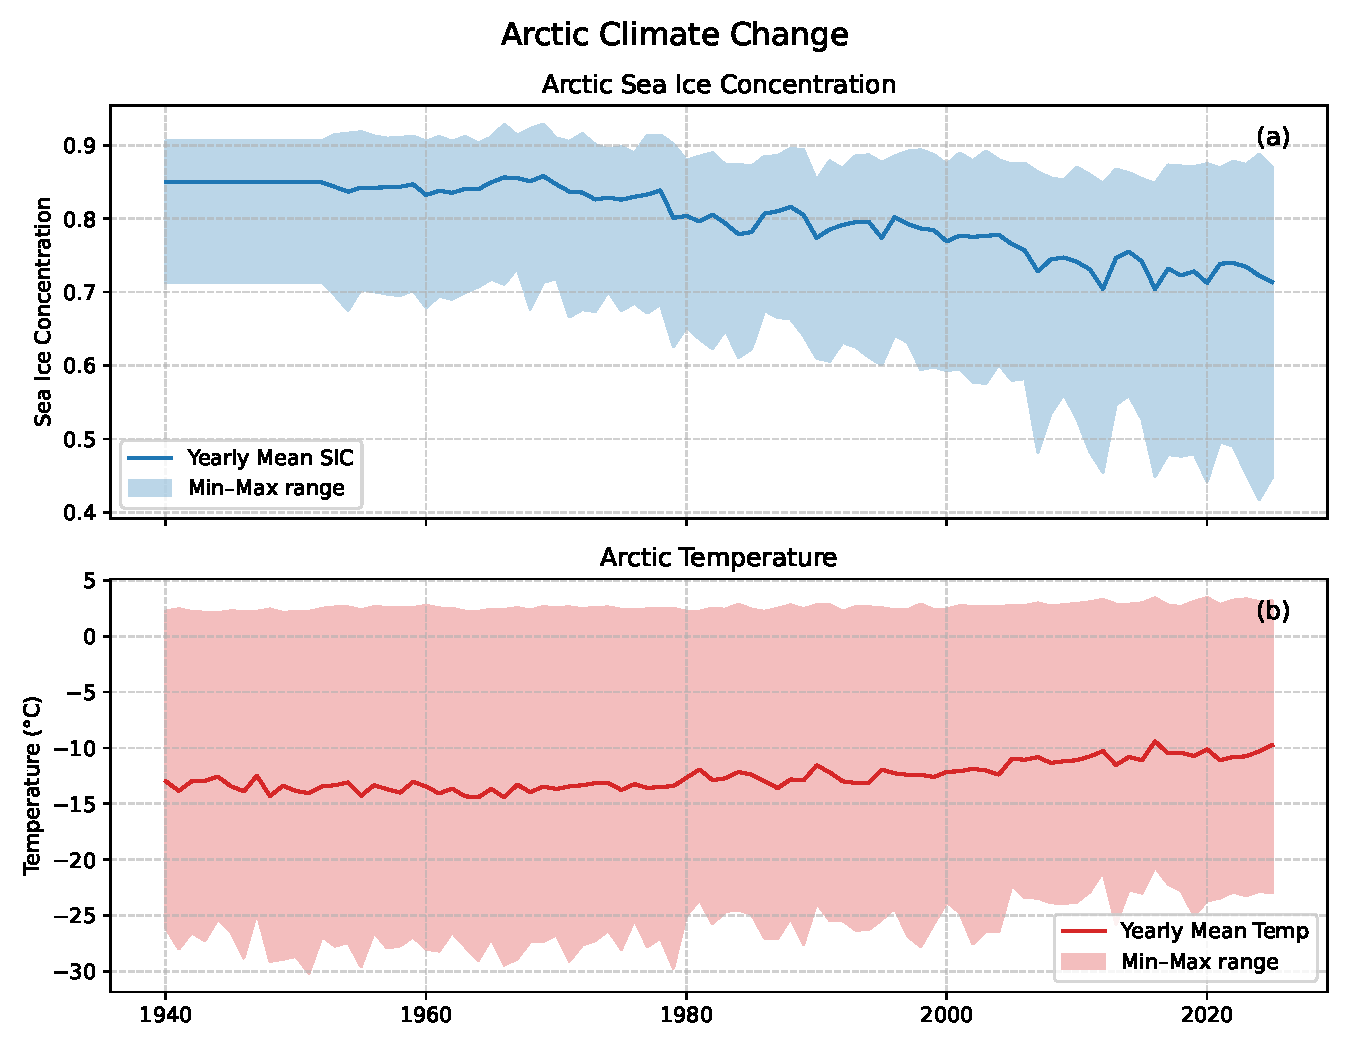
\includegraphics[height=0.7\textheight]{Figures/Arctic-climate-change.pdf}
    \caption{Arctic change in sea-ice concentration and temperature, ERA5 (1940-2025).}
  \end{figure}
\end{frame}



\begin{frame}{Climate Change}
    \begin{spacing}{1.5} 
\begin{itemize}

    \item The Arctic is warming at nearly four times the global average rate (Arctic amplification) \citep{rantanen2022}.
      \item Decline in sea ice extent, reducing albedo and increasing solar absorption.
      \item Thawing permafrost
      \begin{itemize}
        \item Releases greenhouse gases.
        \item Formation of thermokarst $\longrightarrow$ changes in river flow patterns. 
      \end{itemize}
    \item Arctic Ocean may be ice-free during summer by 2050 \citep{hartmann2016}

  \end{itemize}
  \end{spacing}
\end{frame}


\begin{frame}{Societal activities}
    \section{Societal activities}
    \begin{spacing}{1.5} 
  Climate change impacts on societal activities:
    \begin{itemize}
      \item Opening of new shipping routes due to sea-ice retreat.
      \item Increased interest in resource extraction (minerals, oil).
      \item Growing interest from major powers (e.g., the United States) in controlling Arctic routes and resources \citep{CongressionalResearchService2026}.
      \item Potential impacts on Indigenous peoples and the Arctic environment according to \citet{IPCC2023}.
  \end{itemize}
  \end{spacing}
\end{frame}